\documentclass[10pt]{beamer}

\usetheme{default}

\usepackage[utf8]{inputenc}
\usepackage[russian]{babel}
\usepackage[OT1]{fontenc}
\usepackage{amsmath}
\usepackage{amsfonts}
\usepackage{amssymb}
\usepackage{graphicx}
\usepackage{etoolbox}
\usepackage{caption}
\usepackage{subcaption}
\usepackage{pifont}
\usepackage{xcolor}
\usepackage{framed}
\definecolor{shadecolor}{cmyk}{0,0,0,1}
\usepackage{multirow}

\usepackage{listings}

\lstset{
	backgroundcolor=\color{lightgray},
	commentstyle=\color{blue},
	frame=single
	breakatwhitespace, 
	language=python, 
	columns=fullflexible, 
	keepspaces, 
	breaklines, 
	tabsize=3, 
	showstringspaces=false, 
	extendedchars=true,
	numbers=left
}

\makeatletter

\setbeamercolor{title}{fg=white}
\setbeamercolor{frametitle}{fg=black}
\setbeamerfont*{title}{family=\sffamily,size=\LARGE}

\setbeamerfont{page number in head/foot}{size=\scriptsize}
\setbeamertemplate{footline}[frame number]
\let\otp\titlepage
\renewcommand{\titlepage}{\otp\addtocounter{framenumber}{-1}}

\setbeamertemplate{background canvas}{%
	\ifnumequal{\c@framenumber}{0}{%
      
\includegraphics[width=\paperwidth,height=\paperheight]{images/cover.png}
   }{%
      \ifnumequal{\c@framenumber}{\inserttotalframenumber}{
         
\includegraphics[width=\paperwidth,height=\paperheight]{images/back.png}
      }{%
         % Other frames
      }%
   }%
}

\makeatother

\beamertemplatenavigationsymbolsempty

\author{Николай Анохин}
\title{\newline \newline \newline Лекция 11 \\ Data Mining в реальных системах}

\begin{document}

\begin{frame}[plain]
\titlepage
\end{frame}

\begin{frame}{}

\begin{center}
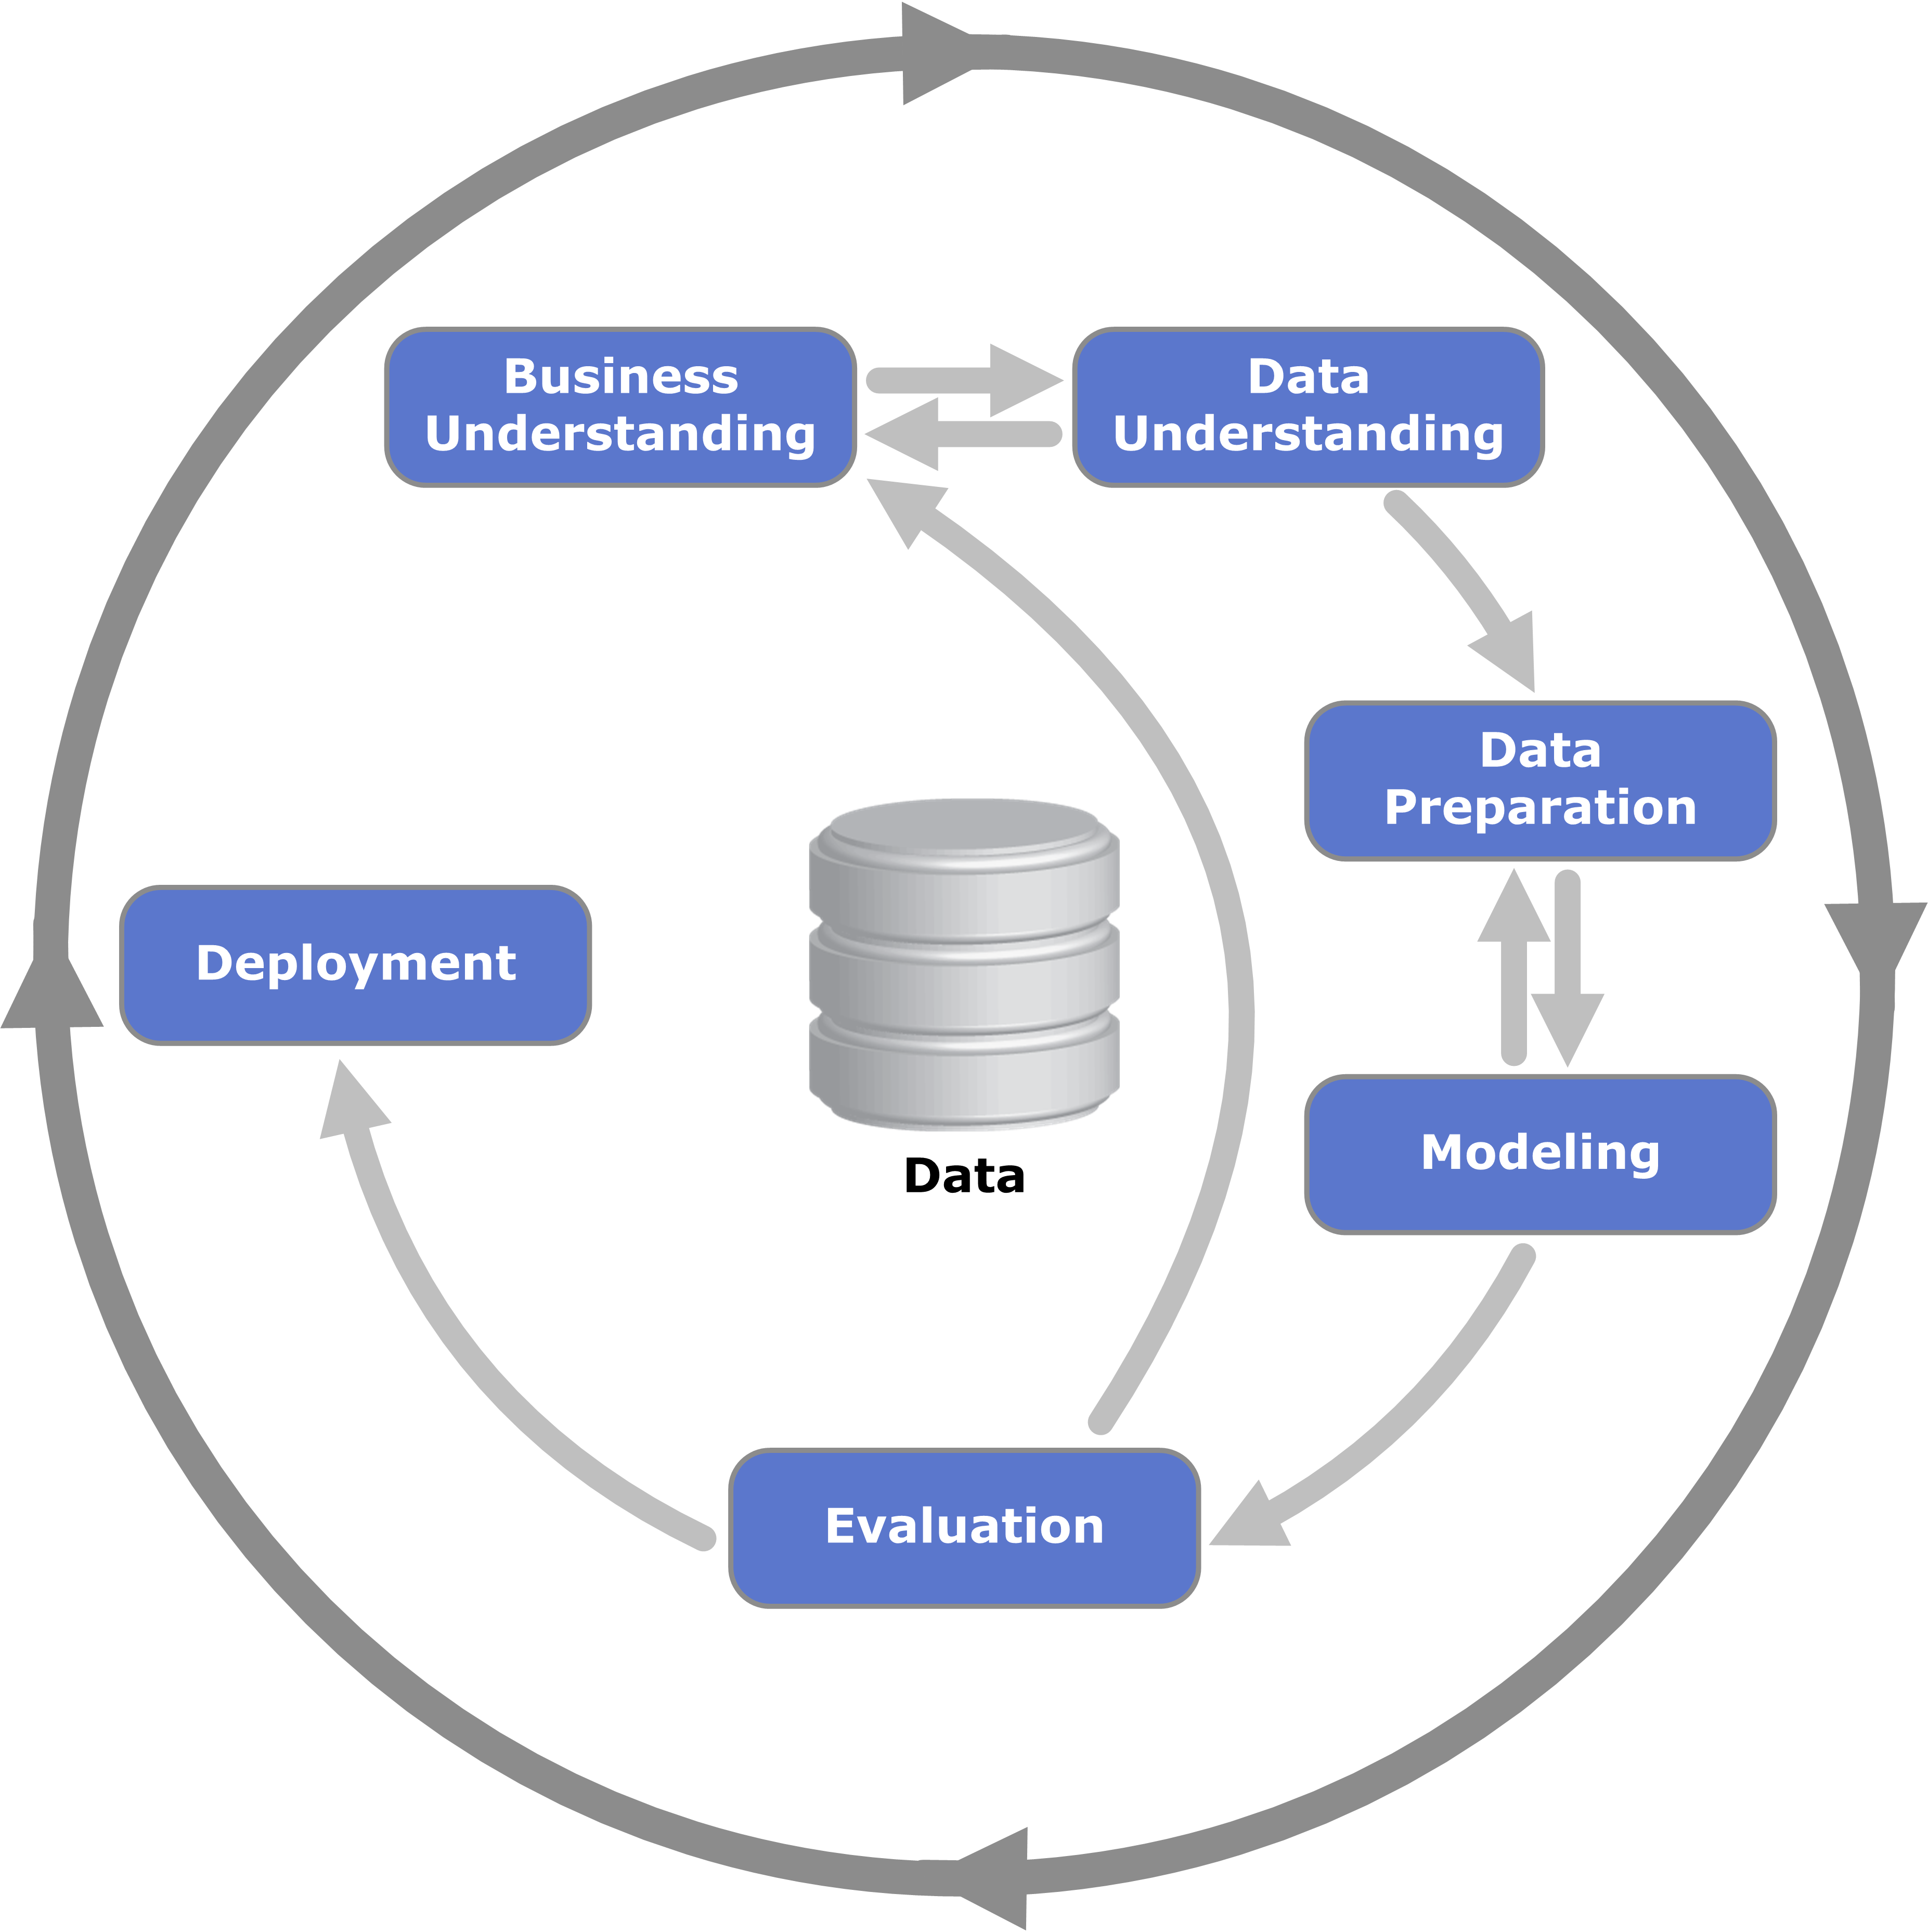
\includegraphics[scale=0.4]{images/crisp.png}
\end{center}

\end{frame}

\begin{frame}{План занятия}
\tableofcontents
\end{frame}

% ============================================== %

\section{Работа с признаками}

% ============================================== %

\begin{frame}{}

\begin{center}
\Large Работа с признаками
\end{center}

\end{frame}

\begin{frame}{Конструирование признаков}

\end{frame}

\begin{frame}{Преобразование признаков}

\begin{itemize}
\item Дискретизация
\item Проекции
	\begin{itemize}
	\item PCA
	\item Random projections
	\end{itemize}
\item Заполнение отсутствующих значений
\item Удаление шума
\end{itemize}

\end{frame}

\begin{frame}{Отбор признаков}

Как ``нерелевантные'', так и ``релевантные'' признаки могут быть вредными

\begin{enumerate}
\item Независимо от алгоритма обучения: backward elimnation, forward selection
	\begin{itemize}	
	\item mutual information	
	\item коэффициент корреляции
	\item линейная модель
	\item генетические алгоритмы
	\end{itemize}
\item С использованием алгоритма обучения (кросс-валидация, hold-out)
\end{enumerate}

\end{frame}

% ============================================== %

\section{Алгоритмы машинного обучения}

% ============================================== %

\begin{frame}{}

\begin{center}
\Large Алгоритмы машинного обучения
\end{center}

\end{frame}

% ============================================== %

\section{Особенности реальных систем}

% ============================================== %

\begin{frame}{}

\begin{center}
\Large Особенности реальных систем
\end{center}

\end{frame}

% ============================================== %

\section{Что дальше}

% ============================================== %

\begin{frame}{}

\begin{center}
\Large Что дальше
\end{center}

\end{frame}

\begin{frame}{}

\begin{center}
\Large Вопросы
\end{center}

\end{frame}

\end{document}